%=========================================================================================================================================
%=========================================================================================================================================
\chapter{Background} \label{chapter:Background}
%=========================================================================================================================================
%=========================================================================================================================================



%-----------------------------------------------------------------------------------------------------------------------------------------
\section{Named Data Networking}
%-----------------------------------------------------------------------------------------------------------------------------------------

%-----------------------------------------------------------------------------------------------------------------------------------------
\subsection{NDN Fundamentals}
%-----------------------------------------------------------------------------------------------------------------------------------------

%hourglass architecture + figure \\
%interest \& data packets + figure \\
%router components and workflow (PIT, FIB, CS) + figure \\

 In NDN communication is driven by the receivers through exchanging two types of packets: \textbf{Interest} and \textbf{Data}. If a consumer wants to receive a chunk of data, he sends out an Interest into the network, which contains the name of the resource that should be acquired. The routers then forward the Interest until it ends up at the producer of said resource. The producer then deletes the Interest and in turn sends out a Data packet, containing the requested content, its name and a signature from the producer's key (Figure \ref{fig:fundamentals:NDNPackagestructure}). 

 \begin{figure}[ht]
 	\centering
 	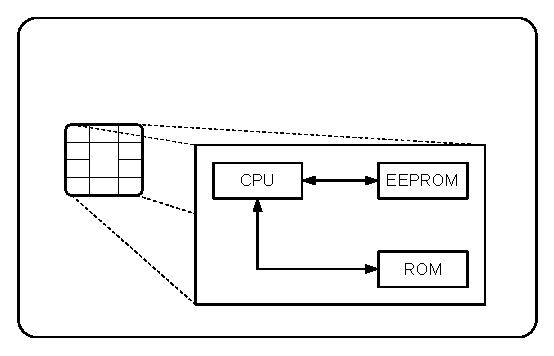
\includegraphics{grundlagen/speicherkarte}
 	\figcaption{Packets in the NDN Architecture. \cite{ZABJ14}}
 	\label{fig:fundamentals:NDNPackagestructure}
 \end{figure}
 
 The Data packet travels back to the consumer, following the reversed path of the Interest that requested it. If the consumer wants further data, he has to send a new Interest. In order for this to work, all NDN routers are equipped with following data structures: A \textbf{Pending Interest Table (PIT)}, a \textbf{Forwarding Information Base (FIB)} and a \textbf{Content Store (CS)}. The PIT is a list containing entries for all Interests that have been forwarded, but not yet satisfied with a Data packet. The FIB has a routing protocol based on name-prefixes and decides where to forward Interests when applicable, following a specific forwarding strategy. The CS is a temporary cache for all the Data packets that recently satisfied Interests. Since an NDN Data packet is meaningful independent from source or destination, it can be distributed by the router itself if the same Data is requested by multiple consumers within a short period of time. Using all these data structures, the forwarding process at an NDN router looks as follows (see also Figure \ref{fig:fundamentals:NDNForwardingProcess}):

 \begin{figure}[ht]
 	\centering
 	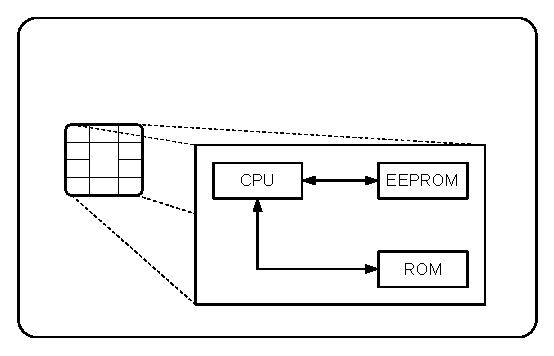
\includegraphics{grundlagen/speicherkarte}
 	\figcaption{ Forwarding Process at an NDN Node. \cite{ZABJ14}}
 	\label{fig:fundamentals:NDNForwardingProcess}
 \end{figure}


When an Interest arrives at the router, the first thing it does is to look if the requested data is already available in the CS. If so, the Interest can be satisfied immediately and the corresponding Data packet is sent back. Otherwise, the router checks if the name contained in the Interest is already saved as entry in the PIT. If it is, someone else has requested the same data but it has not yet arrived. If that is the case, the incoming interface will be added to the PIT entry. If there is no entry yet, a new entry is created and the packet will be forwarded to a node closer to a possible source, which is determined by the FIB via a name-prefix based protocol. If a Data packet arrives at an NDN Router, the PIT is searched for a matching entry. If no entry is found, the data packet will be discarded. Otherwise the Data packet is then duplicated and send to each downstream interface noted there, followed by the removal of said entry from the PIT. The Data is then saved in the CS in case it will be requested again in the near future. This whole process ensures that "routing" is only needed towards the producer of content, since the Data packets simply follow the reversed path of their corresponding Interest. It also ensures that the number of Interest and Data packets stay the same (given that no packets are lost), creating a \textbf{flow balance}, similar to what TCP provides. The key difference here is that TCP was built as an additional layer over IP, while in NDN the flow balance is an in-built feature. In fact, no additional transport layer is required at all, because NDN takes on many of its tasks by itself anyway. The rest (like de-multiplexing, reliable delivery, etc.) will be managed by the applications themselves, if they actually require those features. \cite{ZABJ14}


%-----------------------------------------------------------------------------------------------------------------------------------------
\subsection{NDN Specifics}
%-----------------------------------------------------------------------------------------------------------------------------------------
The following section aims to discuss specific aspects of NDN in further detail. %TODO is this still accurate?

%-----------------------------------------------------------------------------------------------------------------------------------------
\subsubsection{Naming}
%-----------------------------------------------------------------------------------------------------------------------------------------
%Structure of name
%it's hierarchical --> allows scaling
%names/routing unique only within its scope (smart home - global)

%dynamically generated contnt needs names to be constructed deterministically (algorithm, rule)
%partial names + selecter like "leftmost child" also possible

%its' opaque to the network --> independently developed by each app
%freedom for developers/apps to shape naming to their needs
%guidelines and libraries to facilitate naming conventions though

One of the biggest and most characteristic features of NDN is the naming itself. A name in NDN can be used to reference a multitude of things, from a simple command to whole chunks of a video. An example for the latter could look like \textit{"/itec/videos/demo.mp4"}. While not completely necessary, most names in NDN have some sort of hierarchical structure, with different levels separated by a "/", not unlike current URLs. This allows for much easier scaling than flat names, especially considering that namespaces for data that should be available world wide needs unique names on a global scale. There are however also use cases like smart homes where the requirements for uniqueness are significantly smaller, and can be used to map dependencies and relations like in \textit{"/myhome/bedroom/lights/off"}.

In order to request data, the name must first be known to the consumer. While this may be feasible with static content, dynamic content needs names to be constructible deterministically by both consumer and producer. This can be achieved by using algorithms or rules that are known and agreed upon by both parties. Alternatively, Interest selectors in conjunction with longest prefix matching can be used to request data without knowing the full naming structure. For example, the first section of a video might be requested with \textit{"/itec/videos/demo.mp4/"} and the \textit{"leftmost-child"} selector, which the producer could then answer with sending \textit{"/itec/videos/demo.mp4/1/"}.

Despite this breadth of possibilities in naming, the routers do not actually know most of its meaning, which makes the name \textbf{opaque} to the network. This allows the network and application layer to be developed independently from each other and gives developers the freedom to shape naming to the needs of their application. Nevertheless, there are efforts to streamline this process by providing libraries and guidlines to facilitate naming conventions to some degree.
%-----------------------------------------------------------------------------------------------------------------------------------------
\subsubsection{Forwarding}
%-----------------------------------------------------------------------------------------------------------------------------------------

%-----------------------------------------------------------------------------------------------------------------------------------------
\subsubsection{Caching}
%-----------------------------------------------------------------------------------------------------------------------------------------

%-----------------------------------------------------------------------------------------------------------------------------------------
\subsubsection{Security}
%-----------------------------------------------------------------------------------------------------------------------------------------

%-----------------------------------------------------------------------------------------------------------------------------------------
\subsubsection{Mobility}
%-----------------------------------------------------------------------------------------------------------------------------------------

%-----------------------------------------------------------------------------------------------------------------------------------------
\subsection{NDN Limitations}
%-----------------------------------------------------------------------------------------------------------------------------------------
Current obstacles and problems? \\
Current open questions in science?

%-----------------------------------------------------------------------------------------------------------------------------------------
\section{Adaptive Video Streaming}
%-----------------------------------------------------------------------------------------------------------------------------------------
fundamentals used today?

%-----------------------------------------------------------------------------------------------------------------------------------------
\subsection{Adaptive Rate Control}
%-----------------------------------------------------------------------------------------------------------------------------------------
what is that? \\
why is it important?

%-----------------------------------------------------------------------------------------------------------------------------------------
\subsection{Adaption logics}
%-----------------------------------------------------------------------------------------------------------------------------------------
what are those? \\
which are interesting here? \\
present a few.

%-----------------------------------------------------------------------------------------------------------------------------------------
\subsection{Adaptive Video Streaming over HTTP}
%-----------------------------------------------------------------------------------------------------------------------------------------
short description of current TCP streaming (basically DASH)

%-----------------------------------------------------------------------------------------------------------------------------------------
\section{Quality of Experience}
%-----------------------------------------------------------------------------------------------------------------------------------------
what is important for conversational services? \\
end-to-end latency, packet loss...

%-----------------------------------------------------------------------------------------------------------------------------------------
\subsection{Metrics}
%-----------------------------------------------------------------------------------------------------------------------------------------
Discuss those that are going to be used in evaluation later \\
Pro/cons for each metric

%=========================================================================================================================================
%=========================================================================================================================================
% EOF
%=========================================================================================================================================
%=========================================================================================================================================
